\documentclass[11pt]{article}
\usepackage[top=1in,left=1in,right=1in,bottom=1in]{geometry}
\usepackage{graphicx}
\usepackage{multicol}
\begin{document}
\title{\textbf{Project Report}}
\author{Name:Sayeed Hossen Bappy,  Roll:143081}
\maketitle
\begin{multicols}{2}
\section{Abstract}
In this course, I have to develop a web based project. In this purpose I have developed a well needed website that would help me to store my songs and audio stories according to their singer or writer. To make it more user friendly I have added some additional feature like favorite songs or stories, list of all songs and stories, search option for desired songs or stories. In the purpose of public use of my website I have also added log in panel. 
\section{Introduction}
In my website I could store my songs and stories according to their singer or writer. To do so I have an attribute called Albums and an attribute name Songs.
\subsection{Albums}
Here a user could see all the albums with album logo, album title and artist which is uploaded on the website. By clicking on the album one can see which songs is in the particular album.
\subsection{Songs}
This field contains all the songs uploaded on the website according to uploaded time. This field also contains a audio file play button and a favorite tag mark.
\\To make the website more user friendly I have also added some cool feature and they are:
\subsection{Search Option}
This would show user a match result according to what a user tries to find. This process works using *S* method like anything containing the search word would be shown on the result.
\subsection{User Log in}
For public uses of my website, I have added admin panel. That mean anyone can join my website with proper authenticate log in. A logged in user can upload file on the website as like as admin dose.
\section{Necessary Software}
\begin{enumerate}
\item Python 3.6.2
\item Django 1.11.6
\item JetBrains PyCharm Community Edition 5.0.4
\item Browser (Chrome, Firefox)
\item Windows PowerShell / Command Prompt
\end{enumerate}
\section{Programming Languages}
\begin{enumerate}
\item HTML
\item CSS
\item PYTHON(DJANGO)
\end{enumerate}
Also need necessary knowledge in BOOTSTRAP.
\section{Environment Setup}
\subsection{Install Python: Version 3.6.2}
The Python download requires about 30 Mb of disk space; keep it on your machine, in case you need to re-install Python. When installed, Python requires about an additional 90 Mb of disk space.
\subsubsection{Downloading}
\begin{enumerate}
\item Click https://www.python.org/downloads/
\\The following page will appear in your browser.
\begin{center}
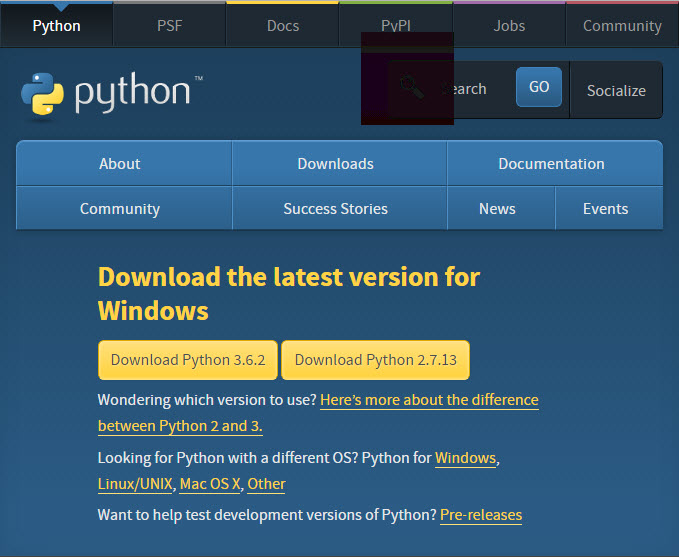
\includegraphics[scale=0.40]{1.jpg} \\ 
\end{center}
\item Click the Download Python 3.6.2 button.
The file named python-3.6.2.exe should start downloading into your standard download folder. This file is about 30 Mb so it might take a while to download fully if you are on a slow internet connection (it took me about 10 seconds over a cable modem).
The file should appear as
\begin{center}
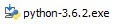
\includegraphics[scale=1.50]{2.jpg} \\ 
\end{center}
\item Move this file to a more permanent location, so that you can install Python (and re-install it easily later, if necessary).
\item Feel free to explore this webpage further; if you want to just continue the installation, you can terminate the tab browsing this web page.
\item Start the Installing instructions directly below.
\end{enumerate}
\subsubsection{Installing}
\begin{enumerate}
\item Double-click the icon labeling the file python-3.6.2.exe.
An Open File - Security Warning pop-up window will appear
\begin{center}

\includegraphics[scale=0.70]{3.jpg} \\ 
\end{center}
\item Click Run.
A Python 3.6.2 (32-bit) Setup pop-up window will appear.
\begin{center}
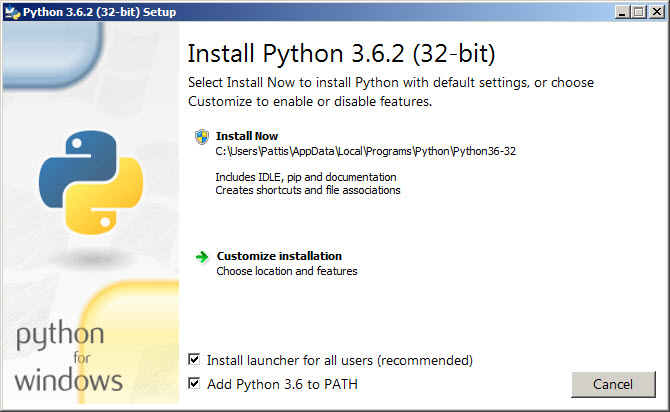
\includegraphics[scale=0.43]{4.jpg} \\ 
\end{center}
Ensure that the Install launcher for all users (recommended) and the Add Python 3.6 to PATH check boxes at the bottom are checked.
If the Python Installer finds an earlier version of Python installed on your computer, the Install Now message will instead appear as Upgrade Now (and the check boxes will not appear).
\item Highlight the Install Now (or Upgrade Now) message, and then click it.
A User Account Control pop-up window will appear, posing the question Do you want the allow the following program to make changes to this computer?
\begin{center}
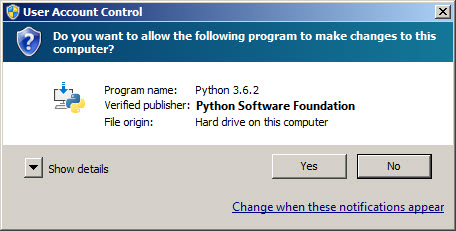
\includegraphics[scale=0.60]{5.jpg} \\ 
\end{center}
\item Click the Yes button.
A new Python 3.6.2 (32-bit) Setup pop-up window will appear with a Setup Progress message and a progress bar.
\begin{center}
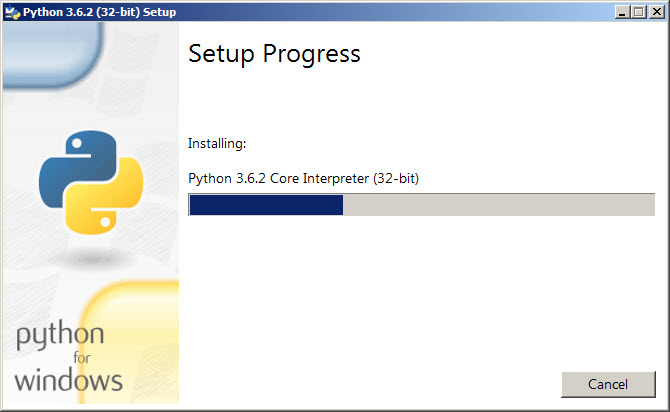
\includegraphics[scale=0.43]{6.jpg} \\ 
\end{center}
During installation, it will show the various components it is installing and move the progress bar towards completion. Soon, a new Python 3.6.2 (32-bit) Setuppop-up window will appear with a Setup was successfully message.
\begin{center}
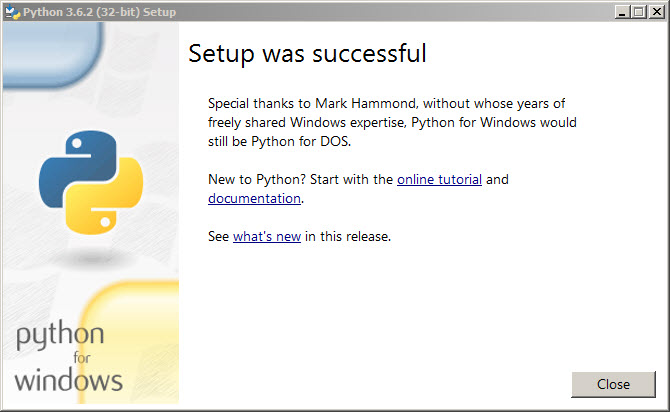
\includegraphics[scale=0.43]{7.jpg} \\ 
\end{center}
Click the Close button.
Python should now be installed.
\end{enumerate}
\subsubsection{Verifying}
To try to verify installation,
\begin{enumerate}
\item Navigate to the directory C:Users/Pattis /AppData/Local/Programs/Python/ Python36-32 (to whatever directory Python was installed:see the pop-up window for Installing step $3$). 
\item Double-click the icon or file python.exe. The following pop-up window will appear.
\begin{center}
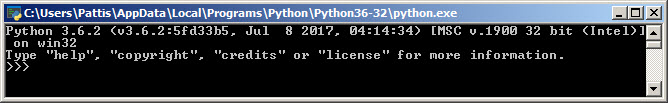
\includegraphics[scale=0.45]{8.jpg} \\ 
\end{center}

\item A pop-up window with the title C:Users/Pattis/AppData/Local/Programs /Python/Python36-32 appears, and inside the window; on the first line is the text Python 3.6.2 ... (notice that it should also say 32 bit). Inside the window, at the bottom left, is the prompt >>>: type exit() to this prompt and press enter to terminate Python.
You should keep the file python-3.6.2.exe somewhere on your computer in case you need to re install Python (not likely necessary).
\\\textbf{Source:} https://www.ics.uci.edu/~pattis/ common/handouts/pythoneclipsejava/ python.html
\end{enumerate}
\subsection{Install Django}
\subsubsection{Install Python}
Django is a Python web framework, thus requiring Python to be installed on your machine. At the time of writing, Python 3.5 is the latest version.
To install Python on your machine go to https://python.org/downloads/. The website should offer you a download button for the latest Python version. Download the executable installer and run it. Check the box next to Add Python 3.5 toPATH and then click Install Now.
After installation, open the command prompt and check that the Python version matches the version you installed by executing:
\\	\textbf{python --version}
\subsubsection{About pip}
pip is a package manage for Python. It makes installing and uninstalling Python packages (such as Django!) very easy. For the rest of the installation, we’ll use pip to install Python packages from the command line.
To install pip on your machine, go to \textbf{https://pip.pypa.io/en/latest/installing/}, and follow the Installing with get-pip.py instructions.
\subsubsection{Install virtualenv and virtualenvwrapper}
virtualenv and virtualenvwrapper provide a dedicated environment for each Django project you create. While not mandatory, this is considered a best practice and will save you time in the future when you’re ready to deploy your project. Simply type:
\\	\textbf{pip install virtualenvwrapper-win}
\\Then create a virtual environment for your project:
\\	\textbf{mkvirtualenv myproject}
\\The virtual environment will be activated automatically and you’ll see “(myproject)” next to the command prompt to designate that. If you start a new command prompt, you’ll need to activate the environment again using:
\\	\textbf{workon myproject}
\subsubsection{Install Django}
Django can be installed easily using pip within your virtual environment.In the command prompt, ensure your virtual environment is active, and execute the following command:
\\	\textbf{pip install django}
\\This will download and install the latest Django release.After the installation has completed, you can verify your Django installation by executing \textbf{django-admin --version} in the command prompt.
\begin{center}
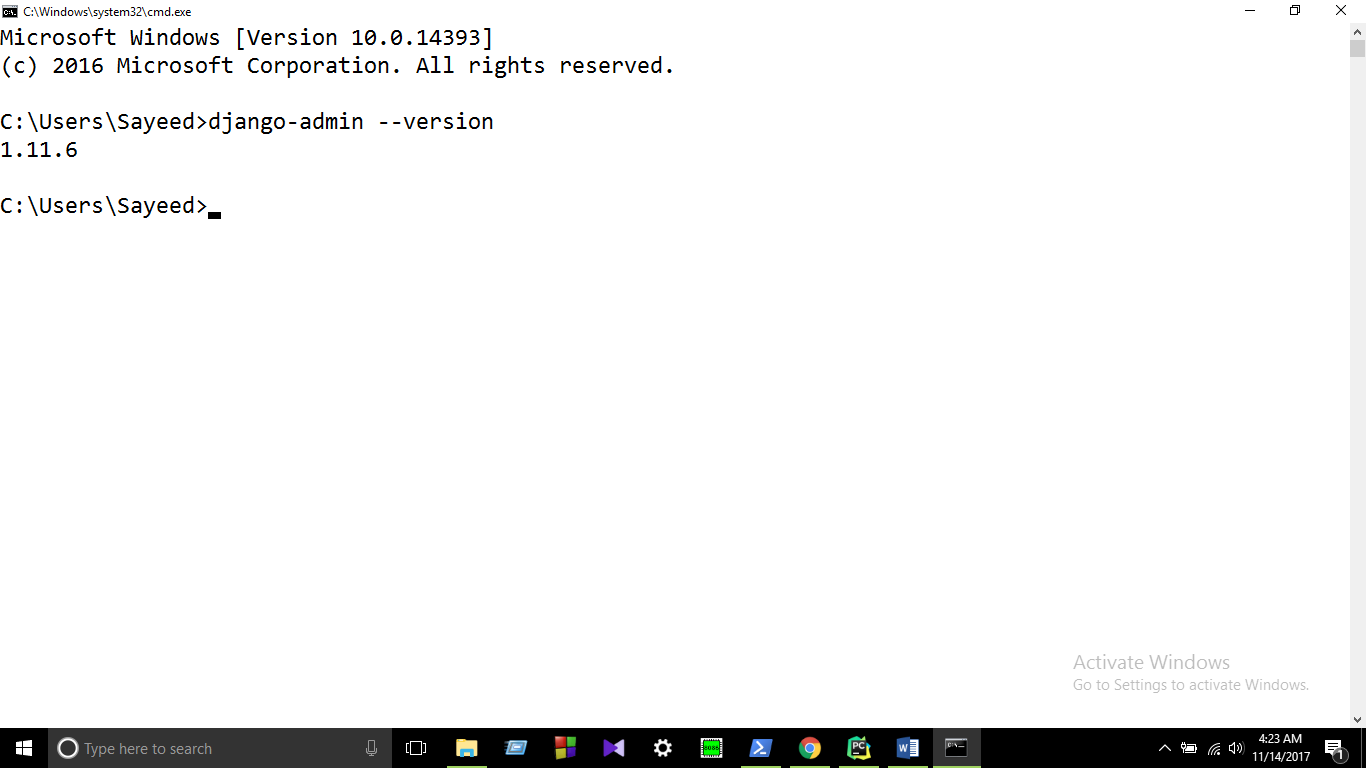
\includegraphics[scale=0.2]{9.png} \\ 
\end{center}
See Get your database running for information on database installation with Django.
\\	\textbf{Source:} https://docs.djangoproject.com/en/1.11/ howto/windows/
\section{Creating a project with Django}
If this is your first time using Django, you'll have to take care of some initial setup. Namely, you'll need to auto-generate some code that establishes a Django project – a collection of settings for an instance of Django, including database configuration, Django-specific options and application-specific settings.
\\From the command line, cd into a directory where you'd like to store your code, then run the following command:
\\	\textbf{django-admin startproject mysite}
\\This will create a mysite directory in your current directory. If it didn't work, see Problems running django-admin.
\subsection{Note}
You'll need to avoid naming projects after built-in Python or Django components. In particular, this means you should avoid using names like django (which will conflict with Django itself) or test (which conflicts with a built-in Python package).
Where should this code live?
\\If your background is in plain old PHP (with no use of modern frameworks), you're probably used to putting code under the Web server's document root (in a place such as /var/www). With Django, you don't do that. It's not a good idea to put any of this Python code within your Web server's document root, because it risks the possibility that people may be able to view your code over the Web. That's not good for security.
Put your code in some directory outside of the document root, such as /home/my code.
\subsection{What is in new project?}
Let’s look at what startproject created:
\\mysite/
    manage.py
    mysite/
        init.py
        settings.py
        urls.py
        wsgi.py
\\These files are:
\begin{enumerate}

\item \textbf{The outer mysite/} root directory is just a container for your project. Its name doesn’t matter to Django; you can rename it to anything you like.
\item \textbf{manage.py:} A command-line utility that lets you interact with this Django project in various ways. You can read all the details about manage.py in django-admin and manage.py.
\item \textbf{The inner mysite/} directory is the actual Python package for your project. Its name is the Python package name you’ll need to use to import anything inside it (e.g. mysite.urls).
\item	\textbf{mysite/init.py:} An empty file that tells Python that this directory should be considered a Python package. If you’re a Python beginner, read more about packages in the official Python docs.
\item	\textbf{mysite/settings.py:} Settings/configuration for this Django project. Django settings will tell you all about how settings work.
\item	\textbf{mysite/urls.py:} The URL declarations for this Django project; a “table of contents” of your Django-powered site. You can read more about URLs in URL dispatcher.
\item	\textbf{mysite/wsgi.py:} An entry-point for WSGI-compatible web servers to serve your project. See How to deploy with WSGIfor more details
\end{enumerate}
\subsection{The development server}
Let’s verify your Django project works. Change into the outer mysite directory, if you haven't already, and run the following commands:
\\	\textbf{python manage.py runserver}
\\You'll see the following output on the command line:
\\	\textbf{Performing system checks...}
\\
\\	\textbf{System check identified no issues (0 silenced).}
\\
\\	\textbf{You have unapplied migrations; your app may not work properly until they are applied.}
\\	\textbf{Run 'python manage.py migrate' to apply them.}
\\
\\	\textbf{November 22, 2017 - 15:50:53}
\\	\textbf{Django version 1.11, using settings 'mysite.settings'}
\\	\textbf{Starting development server at http://127.0.0.1:8000/}
\\	\textbf{Quit the server with CONTROL-C.}
\subsubsection{Note}
Ignore the warning about misapplied database migrations for now; we'll deal with the database shortly.
You've started the Django development server, a lightweight Web server written purely in Python. We've included this with Django so you can develop things rapidly, without having to deal with configuring a production server – such as Apache – until you're ready for production.
Now's a good time to note: don't use this server in anything resembling a production environment. It's intended only for use while developing. (We're in the business of making Web frameworks, not Web servers.)
Now that the server's running, visit \textbf{http://127.0.0.1:8000/} with your Web browser. You'll see a “Welcome to Django” page, in pleasant, light-blue pastel. It worked!
\subsection{Changing the port}
By default, the runserver command starts the development server on the internal IP at port 8000.
If you want to change the server’s port, pass it as a command-line argument. For instance, this command starts the server on port 8080:
\\	\textbf{python manage.py runserver 8080}
\\If you want to change the server’s IP, pass it along with the port. For example, to listen on all available public IPs (which is useful if you are running Vagrant or want to show off your work on other computers on the network), use:
\\	\textbf{python manage.py runserver 0:8000}
\\	0 is a shortcut for 0.0.0.0. Full docs for the development server can be found in the runserver reference.
\textbf{Automatic reloading of runserver}
The development server automatically reloads Python code for each request as needed. You don't need to restart the server for code changes to take effect. However, some actions like adding files don't trigger a restart, so you'll have to restart the server in these cases.
\section{Conclusion}
Using the above machine configuration and software status my project is built. Taking additional help from necessary website and tutorial I have completed a structure of a website. This project helps me to learn web based languages and python as well.
\end{multicols}
\end{document}
